\documentclass[runningheads]{llncs}
%
\usepackage[T1]{fontenc}
\usepackage{graphicx}
\usepackage{booktabs,tabularx}
%
\begin{document}
%
\title{One Matched Control Is Not Enough: Physics-Based Attribution of Deadlock Resolution in Pedestrian Steering Models}
%
\titlerunning{One Matched Control Is Not Enough}
%
\author{Palaash Gang\inst{1}\orcidID{0009-0006-7448-9488} \and
Arjun Veluri\inst{1}\orcidID{0009-0001-5940-3272}}
%
\authorrunning{P. Gang and A. Veluri}
%
\institute{Indus International School, Pune, India\\
\email{palaash.gang@indusschoolpune.com} (corresponding author),
\email{arjun.v@indusschoolpune.com}}
%
\maketitle
%
% generated by tools/make_numbers.py from paper/numbers_registry.yaml; do not edit

%
\begin{abstract}
% TODO: abstract (150--250 words)
\keywords{% TODO: keywords
}
\end{abstract}
%
\section{Introduction}
% Budget 2.0 pages. Fig 1 (hero, raster 600 dpi) placed early.
\begin{figure*}[t]
\centering
% TODO: \includegraphics{figures/fig1}
\caption{}\label{fig:hero}
\end{figure*}
%
\section{Background}
% Budget 2.0 pages.
%
\section{Model and Scenarios}
% Budget 2.5 pages. Table 1.
% generated by experiments/tables/make_table1.py from data/params/model.yaml; do not edit
\begin{table}[t]
\caption{Model parameters as used by the simulator (top) and the two declared modes (bottom). Values are read from the code and listed in \texttt{data/params/model.yaml}.}
\label{tab:params}
\centering\footnotesize\setlength{\tabcolsep}{3pt}
\begin{tabular}{@{}p{1.75cm}p{4.9cm}p{4.9cm}@{}}
\toprule
Agents & \multicolumn{2}{p{9.9cm}}{$m=80$ kg; $v_0\sim\mathcal N(1.34,0.26)$ m/s, $\ge0.5$; $r\sim\mathcal N(0.25,0.03)$ m, $\ge0.15$; $\tau\sim U(0.4,0.6)$ s} \\
Speed--density & \multicolumn{2}{p{9.9cm}}{$v_{\rm eff}=v_0\,\mathrm{clip}[1-e^{-\gamma(1/\rho-1/\rho_{\max})},0.05,1]$, $\gamma=1.913$, $\rho_{\max}=5.4$ ped/m$^2$; $\rho$ = neighbours within $R=3$ m over $\pi R^2$} \\
SFM & \multicolumn{2}{p{9.9cm}}{$A=2000$ N, $B=0.08$ m, $k=1.2\times10^{5}$ kg/s$^2$, $\kappa=2.4\times10^{5}$ kg/(m\,s)} \\
Walls & \multicolumn{2}{p{9.9cm}}{same law per segment, $A_w=A$, $B_w=B$; variants $B_w$, $B_{w,\rm edge}$ (within 0.5 m of the door edge), rounded edge $r=0.1$ m} \\
TTC & \multicolumn{2}{p{9.9cm}}{$k_{\rm ttc}=1.5$, $\tau_0=3$ s, $\tau_{\max}=8$ s} \\
ORCA & \multicolumn{2}{p{9.9cm}}{$\tau_h=5$ s, $\tau_{\rm ORCA}=0.5$ s, speed cap $2v_0$, gate $w_o=1-\sigma(\rho;4,2)$} \\
Crush & \multicolumn{2}{p{9.9cm}}{$k_{\rm crush}=3.6\times10^{5}$, $\kappa_{\rm crush}=4.8\times10^{5}$, gate $w_c=\sigma(\rho;5.5,3)$} \\
Run & \multicolumn{2}{p{9.9cm}}{$\mathrm{d}t=0.01$ s; speed limit $2v_0$; noise $\sigma$ per component, set per experiment; exit at $|x-g|<0.5$ m; deadlock: all $|v|<0.01$ m/s for $10$ s} \\
\midrule
Mode & published-reproduction & corrected-forward \\
\midrule
Integrator & semi-implicit Euler, then clamp; force clip $\pm10^{6}$ N & clamp, then position update; no clip \\
Spawn & uniform, overlaps allowed & rejection, non-overlapping \\
ORCA & as implemented & RVO2-faithful \\
Crush & present in C4 & off \\
Wall corners & sum over segments & convex-union rule \\
\bottomrule
\end{tabular}
\end{table}

%
\section{Mechanism Classes and Their Physical Signatures}
% Budget 2.5 pages. Table 2.
% Table 2: mechanism classes and their physical signatures (Plan §9; plan/CHANGELOG.md C6).
% Cell sources: paper/tables/table2_NOTES.md. Needs \usepackage{booktabs,tabularx} in main.tex.
\begin{table}[t]
\caption{Predicted response of each mechanism class to each probe of a frozen deadlock. ``---'': the probe does not test that class.}
\label{tab:signatures}
\centering
\scriptsize
\setlength{\tabcolsep}{2pt}
\renewcommand{\arraystretch}{1.15}
\begin{tabularx}{\textwidth}{@{}l*{7}{>{\raggedright\arraybackslash}X}@{}}
\toprule
Class
 & Quench
 & Replay, $10^{-9}$\,m
 & $\Delta t$, per-step noise
 & $\Delta t$, $\sqrt{\Delta t}$ noise
 & Rest-drive push, $+$ vs $-$
 & Tilt $b\to-b$
 & Corrected numerics \\
\midrule
P
 & held
 & held
 & held
 & held
 & unchanged
 & unchanged
 & persists \\
L
 & frees, deterministic
 & identical replays
 & no $\Delta t$ dependence
 & no $\Delta t$ dependence
 & $+$ frees, $-$ does not
 & ---
 & persists \\
T
 & frees at random, exponential times
 & replays disagree
 & rate falls as $\Delta t$ grows
 & no $\Delta t$ dependence
 & ---
 & ---
 & persists \\
D
 & frees only beyond $b_f$
 & identical replays
 & no $\Delta t$ dependence
 & no $\Delta t$ dependence
 & ---
 & first out switches side
 & persists \\
N
 & frees or holds, depending on solver details
 & outcome changes under $10^{-9}$\,m
 & ---
 & ---
 & ---
 & ---
 & effect disappears \\
\bottomrule
\end{tabularx}
\end{table}

%
\section{Deadlock Physics}
% Budget 3.5 pages. Figs 2, 3, 4.
\subsection{The Lone-Agent Trap at the Door Edges}
\begin{figure}[t]
\centering
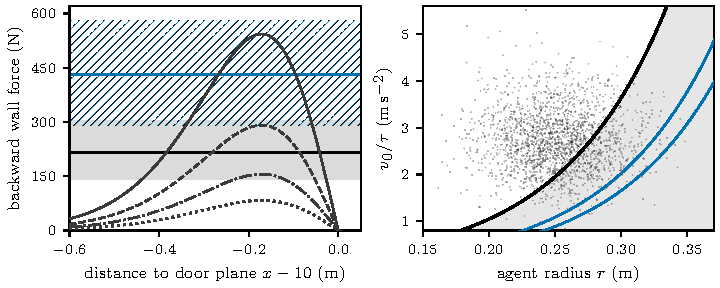
\includegraphics[width=\textwidth]{../figures/fig2_lone_trap.pdf}
\caption{Left: backward wall force on a lone agent on the door axis ($w=0.8$\,m) against distance to the door plane for four radii, with the population drive bands; right: the stuck-alone margin over the $(r,v_0/\tau)$ plane, with the 20\,000 spawned agents. Dark grey curves are $r=0.20$, $0.25$, $0.30$, $0.35$\,m (dotted, dash-dotted, dashed, solid); bands show the 5--95\% range and lines the median of $m v_0/\tau$ for C1 (black) and of the rest-state drive for C3 RVO2 (blue); on the right the margin runs from $-150$\,N (passes alone) to $+150$\,N (held alone) in cividis, the black line is the C1 boundary and the blue band the C3 boundary for $\tau\in[0.4,0.6]$\,s.}
\label{fig:lone-trap}
\end{figure}
\subsection{The Symmetric Pair Standoff}
\subsection{No Persistent Contact Arches}
\subsection{Noise as Collective Activated Escape}
%
\section{Attribution Results}
% Budget 4.0 pages. Figs 5, 6, 7; Tables 3, 4.
\subsection{The Lone Trap}
\subsection{The Pair Class}
\subsection{Revisiting the Conference Findings}
%
\section{Validity Against Human Data}
% Budget 2.0 pages. Fig 8.
%
\section{Discussion}
% Budget 1.5 pages.
%
\section{Conclusions}
% Budget 0.5 pages.
%
\subsubsection*{Main Differences from the Conference Version}
% TODO placeholder
%
\begin{credits}
\subsubsection*{Data and Code Availability}
% TODO placeholder
\subsubsection*{\ackname}
% TODO placeholder
\end{credits}
%
\nocite{gang2026}
\bibliographystyle{splncs04}
\bibliography{refs}
\end{document}
